\section{確率分布と中心極限定理 : 推論の足場をつくる}

  \subsection{問い}

    前章では, 数字の羅列を図にして, データの形を見た.
    80本の映画の視聴回数は, 少ない側に山があり, 多い側へ長く裾を引いていた.
    ジャンルごとに典型値や散らばりの様子も違っていた.

    ただ, 前章の終わりにひとつ問いが残っていた.
    この形は, 手元の80本だけのものなのだろうか.
    別の80本を選び直しても, やはり同じように右へ裾を引くのだろうか.
    取り直したときに結果がどれだけ変わりうるのかが分からないと, 図から読み取ったことがどこまで信用できるのか, 判断のしようがない.

    もっとも, 「取り直しても同じ形か」と問うには, その前に, いま見えている形が言葉で言えていなければならない.
    取り直した結果と見比べて同じか違うかを言うには, 元の形の記述が要るからだ.
    そこでまず, 手元の80本の形を言葉にするところから始める.

  \subsection{素朴な方法と限界}

    形を言葉にするだけなら, 難しいことは何もないように思える.
    前章でも「右に裾が長い」「山は一つ」と書き留めてきたし, それで十分伝わっているようにも思える.
    ためしに手元の80本について, 製作費と評価件数のヒストグラムを\cref{fig:ch04-hist-compare}のように並べてみる.

    \begin{figure}[htbp]
      \centering
      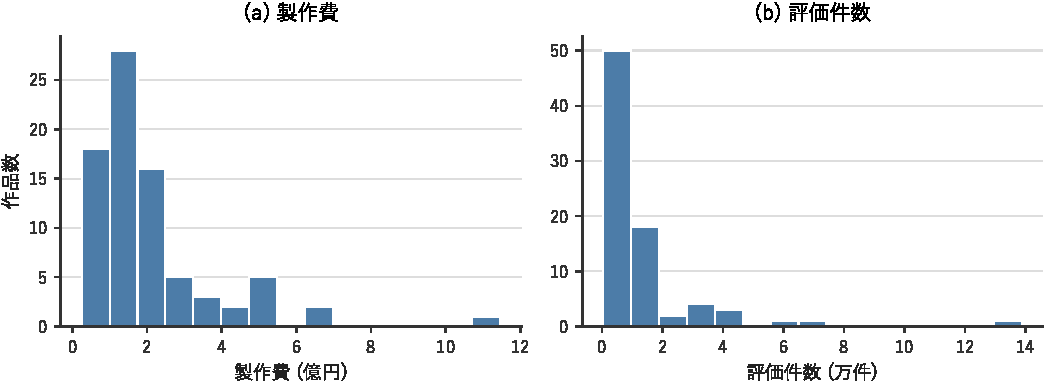
\includegraphics[width=\linewidth]{../figures/output/ch04_hist_compare.pdf}
      \caption{80本の製作費と評価件数のヒストグラム. どちらも右に裾が長いが, 評価件数は少数の作品がとくに大きな値をとる.}
      \label{fig:ch04-hist-compare}
    \end{figure}

    どちらも右に裾が長い.
    しかし並べて見れば, 歪みの程度はまるで違う.
    製作費は, 山のまわりに大半の作品が収まっていて, 裾は緩やかに伸びる程度だ.
    評価件数のほうは, 少数の作品が桁違いに大きく, 裾が横へ長く引き延ばされている.
    「右に裾が長い」という同じひとことに, この二つが同居してしまう.

    そこで, 「かなり長い」「やや長い」と程度を添えてみる.
    ところが, どこからが「かなり」なのかは人によって違う.
    同じ図を見て, ある人は「強く歪んでいる」と言い, 別の人は「少し偏っているだけ」と言うかもしれない.
    程度を測る共通の物差しがないのだ.

    しかも, かりにうまい物差しが見つかったとしても, それで測れるのは手元の80本の形までだ.
    どれほど正確に形容しても今回の標本の描写でしかなく, 「この形は偶然か, それとも仕組みか」を判断する基準は, データの中をいくら見つめても出てこない.

    そうなると, 基準は手元のデータの外に置くしかなさそうだ.
    データの値は, 何もないところから現れたわけではなく, 何かの仕組みから生まれている.
    その仕組みの側から, 形を考えてみる.

  \subsection{理論の最小核}

    \subsubsection*{理論分布 : 仕組みの側から決まる形}

    確率パートで, サイコロの目やコインの表裏を確率変数として扱った.
    サイコロを振る前から, どの目がどれくらい出やすいかは決まっていて, その出やすさの全体を書き表したものが確率分布だった.
    つまり確率分布は, 出た値を集計して得られるものではない.
    値を生む仕組みの側に, はじめから備わっている.

    この見方を, 手元のデータに向けてみよう.
    映画の視聴回数も, 何かの仕組みから生まれた値だと考えられる.
    作品の魅力, 宣伝の規模, 公開のタイミング.
    いろいろな要因が絡み合った結果として, 一本ごとの値が決まっている.
    その仕組みのすべてを書き下すことはできない.
    しかし, もし仕組みのあらましを確率分布のかたちで表せたなら, その分布の形は, 階級の幅にも, どの80本を引き当てたかにも左右されない.
    手元のヒストグラムは, その理論上の形に, 標本ごとの偶然のでこぼこが乗ったものと見なせる.

    このように, データの形の基準として使う確率分布を, \textbf{理論分布}と呼ぶ.
    中身は確率パートで学んだ確率分布そのものであり, 新しい数学が増えるわけではない.
    変わるのは使い方だ.
    確率パートではサイコロのように仕組みが分かっている前提で値の出方を考えたが, ここでは逆に, 目の前のデータの背後にどんな仕組みがありそうかを考えるために使う.

    名前のついた理論分布は, 数えるほどしかない.
    世の中のデータは無数にあるのに, なぜそれで足りるのか.
    それは, 値を生む仕組みのほうに, 共通の骨組みが繰り返し現れるからだ.
    成功か失敗かを何回も数え上げる.
    めったに起きない出来事の回数を数える.
    小さな要因がたくさん足し合わさる.
    こうしたよくある骨組みの一つひとつに, 対応する形が一つずつ付いている.
    分布の名前は, いわば仕組みの名前なのだ.
    代表的な対応は章末のコラム「仕組みから見る理論分布」にまとめたので, 全部を暗記する必要はない.

    そうなると, やることは決まったように見える.
    名前のついた分布の中から手元のデータに合う形を探し当てて, 「視聴回数は〇〇分布に従う」と言えばよい.
    そう言えてしまえば, あとはその分布の性質を使って, 取り直したときに何が起きるかまで計算できそうだ.

    ところが, この道は見かけほど通れない.
    理論分布は, 仕組みを単純化して取り出した理想の形である.
    一方, 視聴回数の背後にあるのは, 書き下すこともできないほど込み入った仕組みだった.
    そんな仕組みから生まれた値が, どれかの理想の形にぴったり従ってくれることは, まずない.
    しかも, かりにぴったり従っていたとしても, 手元にあるのは80本の標本だけで, それを確かめきる手段がない.
    「データは〇〇分布に従う」は, どこまでいっても人間の側の見立てである.
    見立ての上に推論を積めば, 見立てが外れたとき, 積んだ結論ごと崩れる.

    それでも, 見立てがまったくの無駄になるわけではない.
    ぴったりの一致を求めるのをやめて, ヒストグラムと形を見比べ, いま知りたいことに差し支えない程度に近ければ「近い」と言う.
    たとえば「評価件数の分布は対数正規分布に近い」と言えたとする.
    対数正規分布は, たくさんの要因の掛け算が生む, 右に長い裾をもつ理論分布だ(コラム参照).
    この一言で, 聞き手は歪みの程度まで含めて同じ形を思い浮かべられるし, 背後の仕組みについて「掛け算の積み重ねだろうか」という見当まで持てる.
    「右に裾が長い」という感覚頼みの形容が, 基準のある記述に変わる.
    形を語る共通の言葉としてなら, 理論分布は十分に役に立つ.

    ただし, 言葉として役に立つことと, 推論の土台になることは別だ.
    「近い」はあくまで見立てで, その上に「取り直したらどうなるか」の答えを積むわけにはいかない.
    この行き詰まりには抜け方がある.
    ただ, そのためには, 理論分布を一つだけ, 性質までよく知っておく必要がある.
    正規分布だ.

    \subsubsection*{正規分布 : 足し算が生む釣鐘型}

    \textbf{正規分布}は, 左右対称の釣鐘型をした理論分布で, 対応する仕組みは「多数の小さな要因の足し算」である.
    この仕組みが現実にありふれているために, 正規分布はいろいろな場面で繰り返し現れる.

    たとえば人の身長を考えてみる.
    遺伝, 栄養, 運動, 睡眠と, 多数の要因がそれぞれ少しずつ影響して, その積み重ねとして身長が決まる.
    どれか一つの要因が全体を支配することはない.
    こういう成り立ちの量を大勢の人から集めると, 分布は釣鐘型に近づくことが知られている.
    釘を並べた板の上からボールを落とす装置(ゴルトンボード)でも同じことが起きる.
    ボールは釘に当たるたびに左右のどちらかへ小さく逸れ, 着地点は逸れの合計で決まる.
    ボールをたくさん落とすと, 着地点の分布は釣鐘型になる.
    小さなランダムな逸れの足し算, という骨組みが共通しているからだ.

    この釣鐘型を数式で書いたものが, 次の正規分布である.

\begin{defi}{正規分布}{normal_dist}
  確率変数 $X$ が平均 $\mu$, 分散 $\sigma^2$ の\textbf{正規分布}に従うとき, $X \sim N(\mu, \sigma^2)$ と書く.
  その確率密度関数は
  \[
    f(x) = \frac{1}{\sqrt{2\pi\sigma^2}} \exp\!\left( -\frac{(x - \mu)^2}{2\sigma^2} \right)
  \]
  で与えられる.
\end{defi}

    式は見た目より素直にできている.
    まず $(x - \mu)^2$ は, 平均からの距離の二乗だ.
    それがマイナス符号つきで指数関数に入っているから, 平均から離れるほど $f(x)$ は急速に小さくなる.
    つまり, 平均の近くの値ほど出やすく, 遠い値ほど出にくい.
    次に分母の $\sigma$ を見ると, $\sigma$ が大きいほど $(x-\mu)^2$ を割る $2\sigma^2$ が大きくなり, 減り方が緩やかになる.
    山が低く, 裾の広い形になるわけだ.
    逆に $\sigma$ が小さければ, 中心に集中したとがった形になる.
    どこを中心に($\mu$), どれくらいの幅で($\sigma$)散らばるか.
    この2つの数だけで, 正規分布の形は完全に決まる.

    \begin{figure}[htbp]
      \centering
      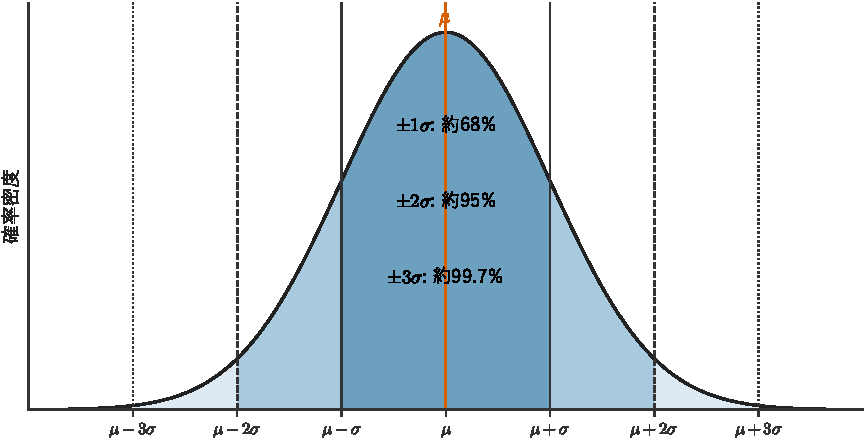
\includegraphics[width=0.9\linewidth]{../figures/output/ch04_normal_ranges.pdf}
      \caption{正規分布で平均から $\pm1\sigma$, $\pm2\sigma$, $\pm3\sigma$ に収まる範囲. 線種と濃淡の両方で境界を示した.}
      \label{fig:ch04-normal-ranges}
    \end{figure}

    形が2つの数で決まるおかげで, 値がどの範囲に散らばるかも, この2つから読み取れる.
    正規分布では, 平均から $\pm 1\sigma$ の範囲に全体の約68\%, $\pm 2\sigma$ に約95\%, $\pm 3\sigma$ に約99.7\%が収まる.
    この割合は $\mu$ や $\sigma$ の値によらず, いつでも同じだ.
    だから, データが正規分布に近いと言えたら, 平均と標準偏差の2つの数を報告するだけで, 聞き手は「値のほとんどがどの範囲にあるか」まで再現できる.
    第2章で学んだ平均と標準偏差は, 分布の形が釣鐘型に近いとき, 数ある要約の中でも特に多くの情報を伝える.
    製造業の品質管理で「寸法が $\pm 3\sigma$ に収まれば合格」という基準が使われてきたのも, この性質をそのまま規格にしたものだ.

    \subsubsection*{取り直したときの平均のばらつき}

    ここで手元のデータに目を戻すと, 少し具合が悪い.
    視聴回数のヒストグラムは右へ大きく歪んでいて, 釣鐘型にはほど遠い.
    実際のところ, 視聴回数, 年収, 評価件数と, 世の中のデータにはむしろ歪んだ形のほうが目につく.
    行き詰まりを抜けるどころか, 正規分布もまた, 手元のデータには当てはまらない理論分布の一つにしか見えない.

    それでも正規分布には出番がある.
    ただし, データそのものの形としてではない.
    それを確かめるために, 前章から持ち越している「取り直したらどうなるか」という問いを, 小さな例で考えてみる.

    ある商品のレビュー評価の平均を知りたいとする.
    レビューは全部で1000件あって, もちろんこの全てを確認できればいいのだが, 残念ながら手元には全体のうち50件しかないとしよう.
    そして, その50件の平均を計算してみると4.2だった.
    では, この計算を基にレビュー全体の平均も4.2と言っていいだろうか.
    もっと言うと, もう一度別の50件を取っても, 平均は再び4.2になるだろうか.
    おそらくそうはならないだろう.
    レビュー全体の平均は4.2とは限らないし, 別の50件を取り直してみたら今度は4.0かもしれない.
    標本を取り直すたびに, 平均は毎回少しずつ違う値になってしまう.

    この事実は当たり前に思えるが, かなり厄介だ.
    手元の4.2という数字が, 本当の平均(母集団の平均なので\textbf{母平均}と呼ぶ)からどれくらい離れているのか分からないからだ.
    1回しか観測していないのに, 「取り直したら毎回違う」という性質にどう対処するのか.
    本章と次章で, この問題にある程度もっともらしい対処法を示していく.

    肝になるのは, 「もし何度も取り直したら, 平均はどんなふうに分布するのか」を考えてみることだ.
    1回ごとの平均の値は予測できなくても, 何度も取り直したときの散らばり方には, 決まったパターンがありうる.
    散らばり方が分かれば, 手元の1回の結果が母平均からどれくらい離れうるのかを見積もる足がかりになる.

    このように, 標本を取り直すたびに統計量を計算し直したとき, その統計量の値が従う分布を\textbf{標本分布}と呼ぶ.

\begin{defi}{標本分布}{sampling_dist}
  母集団から標本を繰り返し取り直し, そのたびに統計量を計算するとき, その統計量の値が従う確率分布を, その統計量の\textbf{標本分布}と呼ぶ.
\end{defi}

    名前がまぎらわしいので, 先に注意しておきたい.
    標本分布は, 手元の標本そのものの分布ではない.
    50件のレビューの星の値がどう散らばっているか, という話なら, それは手元のデータの分布であって, 前章までに見てきたヒストグラムの世界だ.
    標本分布はそうではなく, 「平均」という一つの統計量を, 取り直しのたびに計算し直したとき, その平均の値がどう散らばるか, という分布である.
    データの分布は目の前に描けるが, 標本分布は「もし取り直したら」という仮想の繰り返しを考えて初めて定まる.
    見ている対象がまるで違うので, 混同しないようにしたい.

    ただ, こう定義してみると, 事態は前より苦しくなった気さえする.
    データの分布なら, 少なくともヒストグラムに描いて眺めることはできた.
    標本分布は仮想の繰り返しの上にしか存在しないから, 一度も目に見えない.
    見えるデータの分布でさえ, 理論分布への当てはめは見立ての域を出なかった.
    見えない分布の形など, どうやって知ればよいのか.

    \subsubsection*{中心極限定理 : 平均のばらつきは釣鐘型になる}

    幸い, サイコロのように仕組みを完全に決められる例なら, 「取り直しては平均を計算する」という繰り返しを, 実際にやってみせられる.
    元のデータが歪んでいれば, 平均の散らばり方も同じように歪むと考えるのが自然な気がする.
    それも確かめたいので, わざと偏った例で実験してみよう.

    1の目が出る確率だけが50\%で, 2から6の目は各10\%という, 極端に偏ったサイコロを考える.
    このサイコロを5回振って, 出た目の平均を記録する.
    この「5回振って平均を取る」をまるごと1000回繰り返し, 記録された1000個の平均をヒストグラムにする.

    \begin{figure}[htbp]
      \centering
      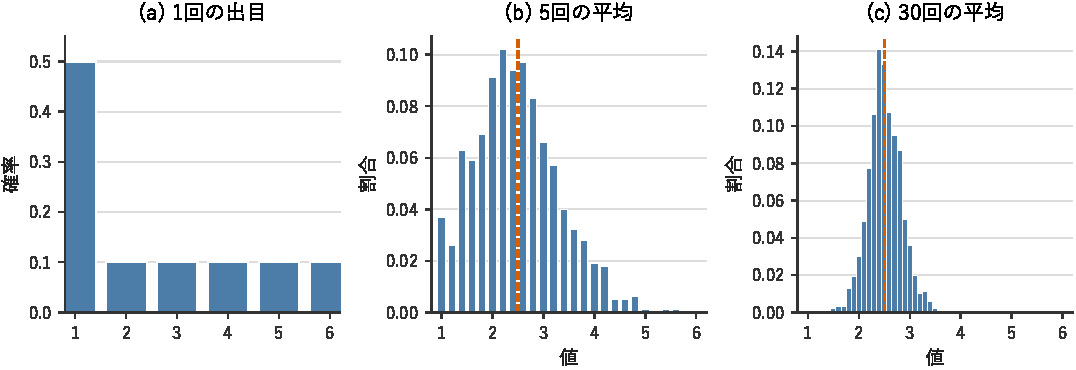
\includegraphics[width=\linewidth]{../figures/output/ch04_dice_clt.pdf}
      \caption{偏ったサイコロの出目と標本平均の分布. 破線は理論上の平均2.5. 5回または30回振って平均を取る操作を1000回ずつ繰り返した. 5回の平均は0.2刻みの値しか取らないため, (b)の棒は櫛状に並ぶ.}
      \label{fig:ch04-dice-clt}
    \end{figure}

    \cref{fig:ch04-dice-clt}を見ると, 5回振りの平均のヒストグラムは, 元のサイコロほどではないにせよ, まだ右に裾を引いた形をしている.
    ところが, 5回を30回に増やして同じことをすると, 平均のヒストグラムはかなりきれいな釣鐘型になる.
    元の分布はどう見ても釣鐘型ではないのに, 平均の散らばり方のほうは左右対称の釣鐘型に近づいていく.
    偶然ではなく, 次の定理が成り立っているためだ.

\begin{thm}{中心極限定理}{clt}
  平均 $\mu$, 分散 $\sigma^2$ をもつ同一の分布から, 互いに独立に $n$ 個の値を取り出し, その標本平均 $\bar{X}$ を計算する.
  $n$ が大きくなるにつれて, $\bar{X}$ の標本分布は正規分布 $N\!\left(\mu,\; \sigma^2 / n\right)$ に近づく.
\end{thm}

    定理の中身を, 部品ごとに確認していく.

    まず前提は, 「同一の分布から, 互いに独立に」の一つだけだ.
    各値が同じ仕組みから生まれていて, ある値の出方が別の値の出方に影響しない, という条件である.
    統計学ではこの条件を\textbf{独立同分布}(i.i.d.: independent and identically distributed)と呼ぶ.
    サイコロの実験なら, 毎回同じサイコロを, 前の結果と関係なく振っていることに当たる.

    次に, 元の分布の形については何も要求していない.
    歪んでいても, 平坦でも, 山が二つあってもよい.
    元のデータがどの理論分布に従うのかを, 見立てる必要すらない.
    i.i.d.でありさえすれば, 平均の標本分布は正規分布へ近づいていく.
    偏ったサイコロの実験で見たのは, まさにこの働きだ.

    「$n$ が大きくなるにつれて」という部分は, 前提条件ではなく, 近づく速さの話である.
    $n$ がいくつ以上なら使ってよい, という境目があるわけではなく, $n$ が増えるほど近似がよくなっていく.
    ただし近づく速さは元の分布の形に左右される.
    元の分布が対称に近ければ $n = 10$ 程度でもかなり釣鐘型に近づくし, 強く歪んでいれば $n = 30$ や $50$ でもまだ歪みが残ることがある.
    「$n \geq 30$ なら大丈夫」という目安を見かけることがあるが, 保証ではなく目安にすぎない.
    元のデータのヒストグラムを見て, 歪みが強いほど $n$ に余裕を見る, というのが実務的な使い方になる.

    そして, 近づく先が $N(\mu,\; \sigma^2/n)$ である.
    中心は元の分布の平均 $\mu$ のままで, 分散が $\sigma^2/n$ に縮んでいる.
    $n$ が大きいほど, 平均の散らばりは小さくなる.
    5件の平均より100件の平均のほうが, 取り直しても安定するはずだという直感と合っている.

    視聴回数のように歪んだデータでは, 正規分布はデータの形の記述としては出番がなかった.
    しかし, そのデータから計算した平均が取り直しでどうばらつくかを考えると, そこには正規分布が現れる.
    それも元の形を問わずに現れるのだから, データが釣鐘型かどうかを心配する必要すらない.

    振り返ると, この章には性格のまるで違う分布が二つ出てきたことになる.
    一つは, データの背後に見立てる理論分布だ.
    「評価件数は対数正規分布に近い」というときの分布で, これは人間の側の見立てであり, 当たっている保証はどこにもなかった.
    もう一つは, 平均という統計量が従う分布だ.
    こちらは見立てではない.
    i.i.d.という前提のもとで, 元のデータがどんな分布だろうと正規分布に近づくことが, 定理として保証されている.
    この後の章で組み立てていく推論は, 「データは〇〇分布に従うはずだ」という当てにならない見立てにではなく, この保証の上に立つ.
    正規分布が統計学の中心に置かれているのも, 釣鐘型のデータが多いからではなく, 統計量のばらつき方というこの土台の側に現れるからだ.

    なお, i.i.d.が崩れている場合, たとえばデータどうしが連動している場合には, この定理はそのままでは使えない.
    そうしたデータへの対処法も研究されているが, 本書ではi.i.d.が成り立つ場合を扱う.

    \subsubsection*{標準誤差 : ばらつきの幅を一つの数にする}

    前の節で見たとおり, 平均の標本分布は正規分布 $N(\mu,\; \sigma^2/n)$ に近づく.
    正規分布の形は, 中心と幅の2つの数で決まるのだった.
    中心は母平均 $\mu$ だから, 残る知りたい量は幅, つまりこの分布の標準偏差である.
    分散が $\sigma^2/n$ なので, 標準偏差はその平方根の $\sigma/\sqrt{n}$ になる.
    取り直したときの平均のばらつきの幅が, この一つの数に集約されている.
    そこで, この量に名前を付ける.

    ただし, 母集団の標準偏差 $\sigma$ は手元から直接は分からない.
    そこで推論では, 手元の標本から
    \[
      u^2 = \frac{1}{n-1}\sum_{i=1}^{n}(x_i-\bar{x})^2, \qquad u = \sqrt{u^2}
    \]
    を計算し, $u$ で $\sigma$ を見積もる.
    $u^2$ は\textbf{不偏分散}, $u$ はその平方根である.
    第2章の $s^2$ は手元のデータを記述するために $n$ で割った量であり, 目的が違う.
    同じデータから計算しても値が少し異なるのは, 第2章の定義が誤りだったからではない.
    なぜ推論では $n-1$ で割るのかは, 検定の数学的背景を扱う章で確かめる.

\begin{defi}{標準誤差}{se}
  母集団の標準偏差を $\sigma$, 標本サイズを $n$ とするとき, 標本平均の\textbf{標準誤差}(SE: Standard Error)を
  \[
    \mathrm{SE} = \frac{\sigma}{\sqrt{n}}
  \]
  と定義する.
  実際には $\sigma$ は未知であるため, 推論用標準偏差 $u$ で置き換えた $\mathrm{SE} = u / \sqrt{n}$ を用いる.
\end{defi}

    定義の後半に断りが入っているのは, $\sigma$ が母集団の値であって, 手元からは分からないためだ.
    その代わりに, 手元の標本から計算した $u$ を使う.
    標本がそこそこ大きければ $u$ は $\sigma$ の代用として使えるので, 本書では以降, $\mathrm{SE} = u/\sqrt{n}$ を標準誤差として使っていく.
    $n$ が小さいときには別に補正のしかたが知られているが, 本書ではデータ数がそこそこ多い場合を扱う.

    式の部品は2つしかない.
    分子の $u$ は, データそのものの散らばりの大きさを推論用に計算した値だ.
    個々の値が大きく散らばるデータほど, 平均も取り直しのたびに大きく動く.
    分母の $\sqrt{n}$ は, 標本サイズの平方根だ.
    件数が多いほど平均は安定する.
    ただし $n$ がそのままではなく $\sqrt{n}$ で効くので, SEを半分にしたければ $n$ は4倍必要になる.
    データを増やせば平均の精度は上がるが, 件数に比例してどこまでも上がるわけではない, ということもこの式から読み取れる.

    名前も式も標準偏差(SD)とよく似ているので, 区別をはっきりさせておこう.
    SDは, 個々のデータが平均のまわりにどれくらい散らばっているかを表す.
    第2章から使ってきた, データの散らばりの指標だ.
    一方SEは, 平均という統計量が, 標本の取り直しに対してどれくらいばらつくかを表す.
    測っている対象が, 個々のデータと統計量とでまるで違う.
    $n$ が大きくなってもSDはほぼ一定のままだが, SEは $\sqrt{n}$ に反比例して小さくなっていく, という振る舞いの違いにも, 対象の違いが表れている.

    「取り直したら結果はどれだけばらつくのか」という冒頭からの問いに, 平均についてはこう答えられる.
    ばらつきの形は正規分布に近づき, 幅は $u/\sqrt{n}$ という一行の計算で見積もれる.
    実際に取り直しを繰り返す必要はなく, 手元の標本が1組あれば計算できる.

  \subsection{手法}

    \subsubsection*{前提条件}
    \begin{itemize}
      \item 観測値が独立同分布(i.i.d.)であること. すなわち, 各観測値が同じ仕組みから生まれ, 互いに影響しないこと.
    \end{itemize}

    前提はこの1点である.
    「$n$ が大きいこと」は前提には入れていない.
    $n$ の大きさが左右するのは正規分布への近さ, つまり近似の精度であって, 手順が使えるかどうかの境目ではないからだ.
    元のデータの歪みが強いほど, 近似の精度には余裕を見ておく.

    \subsubsection*{手順}

    \textbf{Step 1. 形を確認する.}
    ヒストグラムを描き, 山の数, 対称性, 裾の長さ, 外れ値の有無を見る.
    章末のコラムの対応を手がかりに, 近そうな理論分布があれば見当を付けておく.
    強い歪みや極端な外れ値があれば, $n$ とのバランスで正規近似の精度が粗くなることを頭に入れておく.

    \textbf{Step 2. 平均 $\bar{x}$, 推論用標準偏差 $u$, 件数 $n$ を確認する.}
    平均と件数に加え, $n-1$ で割る不偏分散から $u$ を計算する.

    \textbf{Step 3. SEを計算する.}
    \[
      \mathrm{SE} = \frac{u}{\sqrt{n}}
    \]
    これで, 平均を取り直したときのばらつきの幅が見積もれた.

    報告や記録には, 平均とあわせてSEと $n$ を書き添える.
    このときSDとSEを取り違えないよう注意する.
    データそのものの散らばりを伝えたいならSD, 平均がどれだけ安定して求まっているかを伝えたいならSEであり, 両方書くのが親切だ.

  \subsection{実践}

    ランニング例に戻ろう.
    手元にあるのは, 配信サービスの対象作品から抽出された80本の視聴回数だった.
    まず, 中心極限定理が実際に成り立つ様子を確かめ, そのあと手元の平均のSEを計算する.

    \subsubsection*{平均の散らばりを目で見る}

    手元の80本は, サービス全体の対象作品の一部だった.
    もし同じような調査をもう一度行えたら, 平均視聴回数は今回と同じ値になるだろうか.
    実際に調査を何度もやり直すことはできないが, その様子に近いものなら, 手元の80本を使った実験で再現できる.
    まず, 80本のどれも同じ確率で選ばれる仮の分布を作り, 対象作品全体の代わりに使う.
    本数を増やすと平均の散らばりがどう変わるかをあとで見比べるため, まずは少なめの20本で試す.
    この仮の分布から20本を選ぶときは, 一度選んだ作品も候補に戻してから次を選ぶ.
    そのため, 1回の中で同じ作品が複数回選ばれることもある.
    この選び方を\textbf{復元抽出}と呼ぶ.
    20本の平均を計算する操作を1000回繰り返し, 1000個の平均をヒストグラムにする.

    ただし, この実験はサービス全体から20本を本当に取り直す操作と同じではない.
    手元の80本を母集団の代役にした近似であり, 80本の抽出に偏りがあれば, その偏りも引き継ぐ.

    \begin{figure}[htbp]
      \centering
      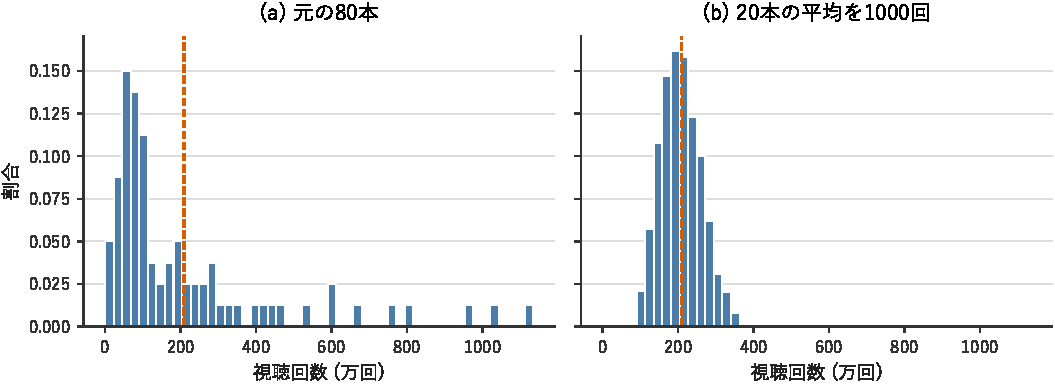
\includegraphics[width=\linewidth]{../figures/output/ch04_sampling_dist.pdf}
      \caption{元の80本の視聴回数と, 80本から20本を復元抽出して求めた標本平均の分布. 復元抽出と平均の計算を1000回繰り返した. 横軸と縦軸の尺度は左右で共通で, 破線は80本の平均を示す.}
      \label{fig:ch04-sampling-dist}
    \end{figure}

    \cref{fig:ch04-sampling-dist}の左側にある元の視聴回数の分布は, これまで見てきたとおり右へ大きく歪んでいる.
    ところが, 20本ずつの平均のヒストグラムは, 左右対称の釣鐘型にかなり近い.
    しかも, 散らばりの幅は元のデータよりずっと狭い.
    歪んだデータからでも, 平均の散らばり方は釣鐘型になる.
    前の節で定理として確認したことが, 手元の80本を使った実験にも表れている.

    \subsubsection*{80本の平均にSEを添える}

    実験で見たのは, 20本ずつ選んだときの平均の散らばりだった.
    一方, 実際に手元にあるのは80本の標本が1組であり, 知りたいのはこの80本の平均のばらつきである.
    件数が違うからといって, 実験を組み直す必要はない.
    SEの式は $n$ の値に応じて幅を見積もれるから, $n = 80$ を入れればよい.
    件数が20本の4倍あるので, $\sqrt{n}$ の働きにより, 幅は実験で見た散らばりのおよそ半分になるはずだ.

    実際に計算してみよう.
    80本の視聴回数について, 平均 $\bar{x}$ はおよそ $209.4$ 万回だった.
    同じ80本から推論用標準偏差 $u$ を計算すると, およそ $240.8$ 万回となる.
    件数は $n = 80$ なので, SEは
    \[
      \mathrm{SE} = \frac{u}{\sqrt{80}} \approx \frac{240.785}{8.944} \approx 26.921
    \]
    となり, およそ $26.9$ 万回になる.

    この数字の読み方を確認しておこう.
    SDである $u$ は, 一本一本の作品の視聴回数がどれだけ散らばっているかを推論用に見積もった値である.
    一方SEは, もし同じ条件で80本の調査を取り直したら, 平均がどの程度動きうるか, という見積もりだ.
    $\sqrt{80} \approx 8.9$ で割っているから, SEはSDの9分の1ほどしかない.
    一本一本の値は大きくばらつくのに, 80本まとめた平均はその何分の一かの幅にしか散らばらない.
    平均という統計量の安定ぶりが, この2つの数字の開きに表れている.

    ただし, この見積もりが頼れるのは, 80本がi.i.d.に近い状況で選ばれている場合だ.
    第1章で置いた「この80本を対象作品全体から大きな偏りなく抽出された標本として扱う」という仮定が, ここで効いている.
    もし抽出に偏りがあれば, SEがいくら小さくても, 平均そのものが母平均からずれた場所に集まってしまう.
    SEが見積もるのは取り直しによるばらつきであって, 偏りの大きさではない.

  \subsection{結果と次の一手}

    出発点は, 「手元で見えた形は, 取り直しても残るのか」という問いだった.
    形を感覚に頼らず語るために理論分布を導入すると, 形の背後にある仕組みごと語れる共通の言葉にはなった.
    しかし, 現実のデータがどれかの理論分布にぴったり従うことは期待できず, 「データは〇〇分布に従う」という見立てを推論の土台にはできなかった.

    突破口は, 問う相手をデータの分布から統計量の分布に替えたことだった.
    手元のデータが歪んでいても, 平均を取り直したときの散らばり方は, i.i.d.のもとで正規分布に近づく.
    これは見立てではなく中心極限定理が保証する事実であり, その散らばりの幅が標準誤差 $\mathrm{SE} = u/\sqrt{n}$ だった.
    手元の標本1組から, 「取り直したら平均はこの程度動きうる」という見積もりが一行の計算で出せる.
    前章まで, 手元の80本について言えることは80本の中で閉じていた.
    いまは, 取り直したらどうなるかという手元の外側への見通しが, 初めて数字になっている.

    ただ, 実際の報告の場面を考えると, もう一歩足りない.
    「平均はおよそ何回, SEはおよそ何回」と伝えられた相手は, その平均をどこまで信用してよいのか, まだ読み取りにくい.
    足りないのは, SEという散らばりの目安を, 誰が読んでも同じ意味になる「幅」のかたちに直す手続きだ.
    その手続きと, 直した幅の正しい読み方が, 次章の主題である.

  \begin{mybox}{コラム : 仕組みから見る理論分布}
    理論分布はたくさんあるが, 全部を覚える必要はない.
    値を生む仕組みの見当が付けば, 候補は自然としぼれる.

    成功か失敗かが決まる試行を $n$ 回繰り返した成功回数なら\textbf{二項分布}.
    めったに起きない出来事が一定期間に起きる回数なら\textbf{ポアソン分布}(平均と分散がほぼ等しいのが目印).
    次に起きるまでの待ち時間なら\textbf{指数分布}(右に長い裾をもつ).
    多数の小さな要因の\textbf{足し算}なら\textbf{正規分布}(釣鐘型).
    多数の要因の\textbf{掛け算}なら\textbf{対数正規分布}(右裾が非常に長い. 対数を取ると釣鐘型に近づく).

    見比べると, 正規分布はほかの型ともつながっている.
    二項分布の成功回数は1回ごとの結果(0か1)の足し算なので, $n$ が大きくなると釣鐘型に近づく.
    掛け算の仕組みも, 対数を取れば足し算に変わるから, 対数の世界では正規分布が現れる.
    いろいろなデータで釣鐘型が見つかるのは, 「足し算」という骨組みがそれだけありふれているからだ.
    最終的には, ヒストグラムを描いて形を目で確かめる.
  \end{mybox}

  \begin{mybox}{コラム : ケトレーとスコットランド兵士の胸囲}
    19世紀, ベルギーの統計学者ケトレー(Quetelet)は, スコットランド兵士5738人の胸囲データを分析し, その分布が正規分布に驚くほどよく合うことを見いだした.\footnotemark
    人体の寸法が多数の小さな要因の和で決まることの, 初期の実証例である.
    しかし, ケトレーは「平均人(l'homme moyen)」という理想像にこだわりすぎた.
    分布の中心から離れた人を「異常」と見なし, 正規分布をあるべき姿の基準にしてしまったのだ.
    正規分布は形を記述するための言葉であって, データや人をその型に押し込む根拠ではない.
    ケトレーの功績と過ちは, この区別を忘れないための教訓になる.
  \end{mybox}
  \footnotetext{%
  Quetelet, A. (1846). \textit{Lettres sur la th\'eorie des probabilit\'es}. Bruxelles: Hayez. 胸囲データの分析はこの書簡集による.}
